\documentclass[
  aps,
  reprint,
  superscriptaddress,
  floatfix,
  nofootinbib,
  longbibliography
]{revtex4-2}

\usepackage{amsmath,amssymb}
\usepackage{graphicx}
\usepackage{xcolor}
\usepackage{tikz}
\usetikzlibrary{calc,positioning,arrows.meta}
\usepackage{hyperref}

\hypersetup{
  colorlinks=true,
  linkcolor=blue,
  citecolor=blue,
  urlcolor=blue
}

% --- convenience macros -------------------------------------------------
\newcommand{\R}{\mathbb{R}}
\newcommand{\E}{\mathbb{E}}
\newcommand{\Prob}{\mathbb{P}}
\newcommand{\Sph}[1]{S^{#1}}
\newcommand{\Msem}{M}
\newcommand{\sint}{\sigma_{\mathrm{int}}}
\newcommand{\Eint}{E_{\mathrm{int}}}
\newcommand{\T}{^{\mathsf{T}}}
\newcommand{\opnorm}[1]{\lVert #1 \rVert_{\mathrm{op}}}
\newcommand{\norm}[1]{\lVert #1 \rVert}

\DeclareMathOperator*{\argmax}{arg\,max}
\DeclareMathOperator{\spanop}{span}
\DeclareMathOperator{\Var}{Var}

\begin{document}

\title{Geometric Limits on Semantic Expressibility: Quantum-Inspired Contexts and Polysemy in Large Language Models}

\author{Karl Svozil}
\email{karl.svozil@tuwien.ac.at}
\affiliation{Institute for Theoretical Physics, TU Wien,
Wiedner Hauptstra\ss{}e 8--10/136, 1040 Vienna, Austria}

\date{\today}

\begin{abstract}
A fixed-width language-model representation may support a semantic-feature
dictionary far larger than its exact carrier dimension.  Let $d$ be the rank
of a declared real carrier, fix an absolute-inner-product tolerance
$0<\varepsilon<1$, and let $M_\varepsilon(d)$ be the maximum cardinality of a
unit-vector family in $\R^d$ whose absolute pairwise inner products do not
exceed $\varepsilon$.  L\'evy concentration explains why almost every
direction is nearly orthogonal to any fixed direction.  The
Johnson--Lindenstrauss lemma gives the complementary finite-set statement:
logarithmic dimension suffices to preserve a prescribed finite geometry, and
its standard-basis construction gives the existence bound
$M_\varepsilon(d)\geq\exp(c\varepsilon^2d)$ for fixed $\varepsilon$ and
sufficiently large $d$.  Direct random spherical coding gives the same
exponential scale, while the Welch bound supplies a deterministic coherence
floor.  If an independently justified full tensor-product carrier has
$d=q^n$, with fixed $q>1$, this becomes
$M_\varepsilon(q^n)\geq\exp(c\varepsilon^2q^n)$, doubly exponential in the
factor count $n$.  For an ordinary Transformer residual stream, however, only
this ambient-code existence result in measured $d$ follows; whether a learned
dictionary approaches it is empirical, and tensor-product growth is an
additional hypothesis.

Geometric coexistence is not the same as simultaneous semantic access.  For
$k$ random-like active directions, a fixed-target correlation readout has
interference of order $\sqrt{k/d}$.  More specifically, learning should place
smaller overlaps between important features that frequently coactivate,
reducing coactivation-weighted interference relative to isotropic and
activity-matched controls.  On this classical geometry we formulate a
separate model of lexical ambiguity: context operators share a token-associated
invariant sector and differ on sense subspaces in its orthogonal complement.
Under spectral separation, the corresponding observables share the projector
onto that sector as a spectral projector.  A learned non-oracular router
selects or mixes the associated linear filters.
The model is quantum-inspired rather than physically quantum, and its content
is the testable advantage of this shared-sector constraint over
parameter-matched classical alternatives on held-out data.
\end{abstract}

\maketitle


% ======================================================================
\section{Introduction}
\label{sec:intro}
% ======================================================================

This chapter examines contextual representation in large language models
(LLMs) as part of the volume's broader inquiry into ``quantum thinking.''
Only a minimal orientation to LLM operation is needed here.  Input text is
first divided into tokens, and each token is mapped to an initial vector.
Transformer blocks then use self-attention and feed-forward transformations
to turn those initially context-free vectors into sequence-dependent hidden
states~\cite{Vaswani-2017-Attention}.  An output layer converts the final state into token scores, and a
softmax distribution supports probabilistic next-token selection.  This
compact chain---tokens, embeddings, contextual transformation, and finite
readout---supplies the computational background for the argument below.
Section~\ref{sec:llm-loops} expands it in plain language and distinguishes
persistent model weights, transient attention coefficients, contextual hidden
states, and optional online updates.  Appendix~\ref{app:llm-loops} gives the
corresponding minimal formalization.

Current Transformer-based LLMs are classical computational systems.  They
run on classical hardware and use real-valued matrix operations,
normalization, nonlinearities, copying, and generally irreversible updates.
Their reliance on vectors, inner products, high dimension, or probabilistic
output does not by itself make them quantum or even quantum-like.  The more
limited question pursued here is where ordinary high-dimensional geometry
already explains the coexistence and contextual selection of semantic
features, and where a stronger comparison with quantum-like formalisms might
begin.  Such a comparison would have to do more than rename familiar neural
operations: it would need to identify a role for contextual bases or subspaces,
incompatible or noncommuting alternatives, interference, or
measurement-like readout that yields explanatory or predictive value beyond
a classical dynamic-embedding account.

Semantic concurrency makes this boundary concrete.  A model must preserve
many latent possibilities while making only a small, context-selected subset
operationally accessible.  Throughout this chapter, \emph{semantic
expressibility} means the number and range of task-relevant distinctions that
remain recoverable under a declared feature extractor, activity distribution,
decoder, and error tolerance.  A large collection of vectors alone is not
semantic expressibility.

Lexical ambiguity is the simplest illustration: the same token can
participate in financial, river-edge, or seat/bench uses of ``bank,'' yet the
surrounding sequence drives it toward different contextual representations.
The umbrella includes both related polysemous senses and historically distinct
homonymous uses~\cite{pustejovsky1995}; the formal construction does not depend
on that lexicographic classification.  This relation among possibility,
context, and readout
connects directly to the volume's recurring themes without implying that the
underlying machine is physically quantum.  It also motivates a separation
between what a representation can geometrically accommodate and what a
finite channel can reliably recover.



The argument has three evidential levels.  First, L\'evy concentration,
Johnson--Lindenstrauss (JL) dimension reduction, spherical coding, and the
Welch bound are established mathematics.  Here they supply complementary
accounts of quasi-dimensionality, not new theorems.  Second, their application
to a learned semantic dictionary is an empirical model whose carrier, metric,
feature extractor, activity distribution, and decoder must be specified.
Third, the shared-sector organization of lexical ambiguity is a stronger hypothesis
tested against classical controls.  No physical quantumness, Born-rule
dynamics, or semantic Kochen--Specker theorem is inferred.

Let $d$ be the exact rank of a declared usable carrier, and let $\Msem$ be the
number of distinct unit feature directions returned by a prespecified
extraction and duplicate-removal rule.  Only $d$ is a vector-space dimension;
$\Msem$ is an empirical dictionary cardinality.  For a fixed amplitude
tolerance $0<\varepsilon<1$, call a family quasi-orthogonal when all absolute
pairwise inner products are at most $\varepsilon$.  L\'evy concentration gives
the typicality statement
%
\begin{equation}
\label{eq:intro-levy}
\Prob\{|u\T x|>\varepsilon\}
\leq 2\exp(-c d\varepsilon^2)
\end{equation}
%
for a fixed unit $u$ and an isotropic random unit $x$.  JL gives a complementary
finite-configuration construction which, after converting distance distortion
to coherence, yields
%
\begin{equation}
\label{eq:intro-jl}
M_\varepsilon(d)\geq\exp(c'\varepsilon^2d),
\end{equation}
%
where $M_\varepsilon(d)$ is the maximum achievable code cardinality under this
condition.  This is an existence result for fixed $\varepsilon$ and
sufficiently large $d$, not a claim that the empirical dictionary size
$\Msem$ attains the bound.

The double exponential requires a second, independent amplification.  If a
carrier has the justified full tensor-product structure
$\bigotimes_{a=1}^{n}\R^q$, with fixed $q>1$, so that $d=q^n$, then
Eq.~\eqref{eq:intro-jl} becomes
%
\begin{equation}
\label{eq:intro-double}
M_\varepsilon(q^n)\geq
\exp\!\bigl(c'\varepsilon^2q^n\bigr),
\end{equation}
%
doubly exponential in $n$ for fixed $0<\varepsilon<1$.  This is a two-stage amplification: composition
first makes the exact carrier exponential, and quasi-orthogonal coding is
exponential in that carrier.  A
standard Transformer residual stream is supplied directly as $\R^d$ and is
not thereby a full tensor product of semantic subsystems.  For LLMs the robust
conclusion is therefore an ambient-code existence lower bound exponential in
measured $d$; the double exponential is a conditional tensor-product
hypothesis.

Abundance also creates crowding.  Among $\Msem$ independently sampled
isotropic directions, the maximum of the $\binom{\Msem}{2}$ pairwise overlaps
is typically
$2\sqrt{\log\Msem/d}$ in the small-overlap regime.  More importantly,
coexistence does not guarantee simultaneous access.  If $k$ random-like
directions are active with order-one amplitudes, a fixed-target correlation
readout accumulates interference
%
\begin{equation}
\label{eq:intro-readout}
\sint\sim\sqrt{\frac{k}{d}}.
\end{equation}
%
The semantic prediction is that learning places smaller overlaps where they
are operationally expensive: between important
features that frequently coactivate.  Coactivation-weighted interference is
therefore compared with isotropic and activity-matched controls.

The chapter finally advances an independent hypothesis about lexical ambiguity.
For some tokens with stable sense inventories, context may be represented by symmetric
operators that share a stable token-associated invariant sector while
differing on low-dimensional sense subspaces in its orthogonal complement.  A
learned router selects or mixes their projections.  Concentration geometry
does not imply this structure; it earns scientific content only if it improves
held-out prediction or compression over parameter-matched unstructured models.
Section~\ref{sec:predictions} states how every layer of the proposal can fail.

A serious caveat is anisotropy.  The nominal width of an LLM layer may exceed
the dimension of the carrier actually occupied by its states.  Throughout this
chapter $d$ therefore means the \emph{usable exact dimension}: first restrict
or whiten the representation to the carrier being tested, then let $d$ be the
size of an orthonormal basis of that carrier.
If this usable $d$ is small, the random-code crowding and readout baselines
worsen.  The
method used to identify the carrier must therefore be declared empirically.

The reference-subspace and operator hypotheses have a narrower domain. They
are meant for lexically ambiguous tokens with established WordNet- or
OntoNotes-style sense inventories and enough SemCor- or WiC-style contextual
evaluation data~\cite{pilehvar2019wic}. Failure on a representative sample,
against the controls in
Sec.~\ref{sec:predictions}, would count against a privileged token reference
subspace or shared-sector operator model even if the broader null calibration
survives.

The proposal is adjacent to the superposition hypothesis in mechanistic
interpretability~\cite{elhage2022superposition}, according to which neural networks
represent more features than they have neurons by packing features into
nearly orthogonal directions. The present chapter separates the
geometric background from a possible semantic organization within it.
The general superposition picture concerns an overcomplete dictionary
of feature directions and sparse active sets. The present model adds the more
specific possibility that contextual readout is organized around stable
token-associated directions and context-dependent, potentially noncommuting
projectors.

Section~\ref{sec:llm-loops} separates creation of the trained weights,
autoregressive response generation, and possible recursive online adaptation.
Section~\ref{sec:concentration} develops the geometric null model through
L\'evy concentration, Johnson--Lindenstrauss dimension reduction, direct
random coding, and the deterministic Welch floor.
Section~\ref{sec:dictionary-readout} separates dictionary coexistence from
simultaneous readout and culminates in the task-dependent criterion of
Sec.~\ref{sec:operating-criterion}. Section~\ref{sec:reference} introduces the
reference-subspace hypothesis, its shared-sector projector and observable
parameterization, and its relation to dynamic contextual embeddings.
Section~\ref{sec:attention} connects the construction to attention as soft
context routing rather than literal basis reconstruction.
Section~\ref{sec:discussion} discusses superposition, sparse
autoencoders, limitations, empirical tests, and the limited quantum
analogy.

\emph{Global variables and local ranks.}
Throughout, $\R^{d}$ is the usable Euclidean carrier, and $d$ is its exact
integer dimension.  The symbol $\Msem$ is the size of a prespecified semantic
feature dictionary; it is a count of directions, not another dimension.  A
dictionary is called overcomplete when $\Msem>d$, and its directions are
called $\varepsilon$-quasi-orthogonal only if their measured overlaps satisfy
the criterion below.  The function $M_\varepsilon(d)$ denotes a
tolerance-dependent code cardinality, not a new dimension.  The symbol $k$
counts directions active in one context.  The optional $n$ counts local
factors only when a full tensor-product structure $d=q^n$ has been independently
specified.  The quantities $\varepsilon$ and the later rms-interference
tolerance $\Delta$ are not dimensions, while $p$ and $m_s$ are local ranks of particular
reference and sense subspaces.  None is a second global vector-space
dimension.  Absolute inner products provide a conservative, sign-insensitive
coherence diagnostic.  When feature orientation carries semantic information,
the signed overlap distribution must be reported as well; no claim that all
semantic features are projective rays is assumed.

The carrier has inner product $u\T v$
and norm $\norm{v}=\sqrt{v\T v}$; $\Sph{d-1}=\{v\in\R^{d}:\norm{v}=1\}$
is the unit sphere; $I$ is the identity matrix; $\opnorm{\cdot}$ is the
operator norm; and $\Prob$ and $\E$ denote probability and expectation under the uniform measure on
the relevant sphere unless stated otherwise. Universal positive
constants are denoted $c,c'$, possibly changing from line to line.

% ======================================================================
\section{From text to weights and back to text: three computational loops}
\label{sec:llm-loops}
% ======================================================================

The word \emph{weight} is used for two different objects in informal accounts
of Transformers.  A trained model has persistent numerical parameters: its
embedding table, query, key, value, output, and feed-forward matrices,
normalization parameters, and final vocabulary readout.  Self-attention also
computes input-dependent coefficients that are often called attention
weights.  Those coefficients exist only for the current forward pass.  They
do not become persistent model parameters.  Keeping this distinction visible
separates the three computational loops below.

\subsection{Creating the weights: tokenization, contextual vectors, and training}
\label{sec:prose-training}

Training begins with text, but a neural network does not receive words or
sentences as primitive objects.  A tokenizer first segments character strings
into a finite vocabulary of token types and replaces each occurrence by an
integer identifier.  Tokens may be whole words, word fragments, punctuation,
spaces, or byte-level units.  Modern subword schemes are designed to cover
rare and previously unseen words without assigning a separate vocabulary
entry to every possible word~\cite{sennrich2016subword,Brown2020May}.  The
tokenizer is normally learned or chosen before the main language-model
optimization and is then held fixed during that optimization.

An embedding table associates each token identifier with an initial real
vector.  At this first lookup stage, two occurrences of the same token use the
same table entry.  Position information is also supplied, either through
added position vectors or through mechanisms such as rotary transformations
inside attention; some systems add role or segment information as well.  The
lookup vector is therefore not yet the fully contextual meaning of that
occurrence.  Context dependence is created by the successive Transformer
layers.

Within one self-attention head, the current vector at each position is mapped
by learned matrices to a query, a key, and a value.  The query at one position
is compared by an inner product with keys at other permitted positions.  In
the decoder-only autoregressive Transformer considered here, a causal mask
excludes future positions during next-token training.  Softmax normalization
turns the permitted comparisons into nonnegative attention coefficients, and
their weighted sum of the value vectors supplies a context-dependent update.
Multiple heads can learn different patterns of dependence.  Residual
connections, normalization, and feed-forward blocks then transform the update
further.  After many layers, the hidden vector for an occurrence of ``bank''
can differ substantially between financial, river-edge, and seat/bench
contexts even though all occurrences began from the same token-table
entry~\cite{Vaswani-2017-Attention}.

This forward calculation still does not create new persistent weights.  The
last hidden state at each training position is converted into scores for the
next token.  The discrepancy between the predicted distribution and the
observed next token defines a training loss.  Backpropagation differentiates
that loss through the output map, feed-forward blocks, attention operations,
and embedding table.  An optimizer then changes the persistent parameters.
Repeating this cycle over many batches creates the trained weight values.  In
short, self-attention produces contextual activations and differentiable
routes through which error signals flow; gradient-based optimization produces
the persistent model weights~\cite{Goodfellow-et-al-2016-Book}.

Does this description require a Hilbert space?  Nothing here requires more
than finite-dimensional Euclidean inner-product geometry.  Because $\R^d$ is
complete, it may formally be called a real Hilbert space, but completeness
plays no computational role and implies no quantum mechanism.  The
construction needs ordinary real vectors, inner products, matrices, and
nonlinear maps; it does not require complex amplitudes, Born probabilities, or
quantum hardware.  Nor does training assign one exactly orthogonal vector to
every token or every meaning.  The quasi-orthogonal geometry studied later
concerns a declared dictionary of extracted feature directions at a chosen
resolution.  It is a possible organization of learned semantic distinctions,
not an assumption built into tokenization or self-attention.

\subsection{Generating an output: tokenization and autoregressive feedback}
\label{sec:prose-generation}

Response generation begins with the same tokenizer.  The prompt, including
any control, role, or formatting tokens exposed to the model, is converted to
a token sequence and then to initial vectors.  The trained parameters are now
normally fixed.  A causal forward pass produces contextual hidden states for
the prompt, and the final relevant state is mapped to one score for every
token in the vocabulary.  Softmax converts these scores into a next-token
distribution.  Greedy decoding chooses its largest entry; sampling may use a
temperature or restrict attention to a high-probability subset before drawing
a token.

The selected token is appended to the sequence.  The enlarged sequence is
then the context for the following prediction, so the generated token can
change all subsequent attention patterns and hidden states.  This loop is
repeated until an end condition is reached.  Implementations commonly cache
previous keys and values to avoid recomputing unchanged parts of the prefix,
but caching changes efficiency rather than the trained parameters.  Finally,
the tokenizer's inverse assembly rules turn the generated token identifiers
back into a character string~\cite{Brown2020May}.

Autoregressive generation is thus already recursive in a precise but limited
sense: each output token becomes part of the next input.  The context,
attention coefficients, and hidden vectors evolve from step to step, while
the persistent model weights remain fixed.  The standard decoding interface
does not require a separately represented complete answer; it emits tokens
successively by repeatedly mapping the current vector-valued context to a
distribution over the next discrete token.

\subsection{Recursive adaptation, alignment, and hallucination}
\label{sec:prose-online}

Three forms of recursion should be separated.  The first is the
autoregressive token feedback just described.  The second adds an external
memory, retrieval result, tool output, or longer conversation history to the
next context without changing the model's persistent weights.  The third is
genuine online learning: after an interaction, a loss or verified feedback
signal updates all parameters, an adapter, or a set of designated fast
weights.  Dynamic evaluation and test-time training show that this third loop
is technically possible~\cite{rannentriki2024dynamic}.  It is not, however,
the ordinary inference rule of the Transformer considered here, and it is not
normally an unrestricted update after every dialogue.

Alignment and safety are among the reasons to constrain such online updates,
but they are not the only reasons.  A user interaction usually supplies no
verified target against which a gradient should be computed.  Unrestricted
updates can cause catastrophic forgetting, distributional drift, loss of
reproducibility, privacy leakage, or deliberate data poisoning through prompt
injection.  Computation and rollback are additional concerns.  A defensible
online learner therefore needs provenance, external verification, bounded or
adapter-local updates, held-out tests, and a recoverable reference model.
Recursive training on unverified model output can instead reinforce errors and
eventually degrade the output distribution~\cite{herel2024collapse}.

The base model produced by next-token pre-training approximates regularities
in its corpus.  Supervised instruction tuning and preference-based methods
then deliberately move the parameters or the effective inference policy
toward chosen notions of helpfulness, harmlessness, instruction following,
and safety~\cite{ouyang2022instructgpt}.  Relative to parameters favored by the
raw next-token objective, this is deliberately an \emph{objective tilt}.
Calling it a geometric distortion would additionally require a declared
parameter-space or output-distribution metric.  In either vocabulary, the
change alone does not imply that factual performance has deteriorated: the
purpose of post-training is to replace the raw objective by a more useful one.

There is nevertheless a concrete version of the concern that alignment can
contribute to hallucination.  If human or learned preferences reward fluent,
confident, accommodating answers more strongly than calibrated abstention,
optimization can favor agreement or plausible completion over epistemic
caution.  Preference judgments have been shown to contribute to sycophantic
behavior in some settings~\cite{sharma2023sycophancy}.  The same pressure could
increase unsupported claims.  Conversely, carefully constructed human
feedback has also improved truthfulness in matched evaluations, and
hallucination already arises in base-model prediction without alignment
post-training~\cite{ouyang2022instructgpt,Kalai2025Why}.  Alignment and factual
accuracy are therefore distinct axes: either can improve while the other
worsens.

The claim that alignment contributes greatly to hallucination should thus be
posed as a causal, model- and protocol-specific hypothesis.  Starting from the
same initialization or base checkpoint, one should compare declared
post-training objectives with matched training data, optimization and compute
budgets, and multiple matched seeds.  Evaluation should use the same prompt
distribution, grounding information, and decoding rule and should measure
unsupported assertions, calibration, coverage, and abstention.  The sign and
magnitude of the change are empirical.  Appendix~\ref{app:online} states this
test without building the desired conclusion into the notation.

% ======================================================================
\section{Quasi-dimensionality from L\'evy concentration and
Johnson--Lindenstrauss}
\label{sec:concentration}
% ======================================================================

The nontrivial question is how the cardinality of a finite-resolution code
scales with its exact carrier dimension.  Here $d$ is the usable carrier rank,
whereas $\Msem$ counts the directions in one measured
dictionary and may exceed $d$.  Let
\begin{equation}
\label{eq:quasiortho}
W=\{w_1,\ldots,w_{\Msem}\}\subset\Sph{d-1},
\qquad
\mu(W)=\max_{i\ne j}|w_i\T w_j|.
\end{equation}
For $0<\varepsilon<1$, we call this particular dictionary
$\varepsilon$-quasi-orthogonal when $\mu(W)\leq\varepsilon$, and write
$M_\varepsilon(d)$ for the maximum cardinality achievable in $\R^d$ under
this condition.  Thus
$M_\varepsilon(d)$ and the empirical count $\Msem$ are cardinalities, not
additional vector-space dimensions.  The term \emph{quasi-dimensionality}
will refer only to this resolution-dependent abundance of directions.

The mathematical ingredients below are established results.  Their purpose
is to distinguish three claims that should not be conflated: L\'evy
concentration says that near-orthogonality is typical relative to a fixed
direction; Johnson--Lindenstrauss (JL) gives a finite-set construction at
logarithmic dimension; and direct random coding provides a null ensemble for
the largest overlap in a dictionary.  None of these facts alone identifies
semantic features in an LLM.

\subsection{L\'evy concentration and angular homogenization}
\label{sec:levy}

In one standard form of L\'evy's lemma, if
$f:\Sph{d-1}\rightarrow\R$ is $L$-Lipschitz in chordal distance and $m_f$ is
a median of $f$, then
\begin{equation}
\label{eq:levy-general}
\Prob\{|f-m_f|\geq t\}
\leq
2\exp\!\left[-c\,\frac{(d-1)t^2}{L^2}\right]
\end{equation}
for a universal constant $c>0$
\cite{ledoux2001concentration,milman1986asymptotic}.  The choice of median or
mean and the numerical constant vary among formulations; the invariant
content is exponential concentration in dimension for every regular scalar
probe.

Fix $u\in\Sph{d-1}$ and take $f_u(x)=u\T x$.  This function is
$1$-Lipschitz and, by rotational symmetry, has median and mean zero.  For
uniform $x\in\Sph{d-1}$,
\begin{equation}
\label{eq:moments}
\E[u\T x]=0,
\qquad
\Var(u\T x)=\frac{1}{d},
\end{equation}
and the corresponding spherical-cap estimate can be written
\begin{equation}
\label{eq:overlap}
\Prob\{|u\T x|\geq\varepsilon\}
\leq
2\exp\!\left[-\frac{(d-1)\varepsilon^2}{2}\right],
\qquad 0<\varepsilon<1.
\end{equation}
Thus almost every direction lies close to the equator perpendicular to a
specified direction, with a typical overlap amplitude of order
$d^{-1/2}$.

There is an equivalent angular description.  If the sign of a direction is
irrelevant, its principal angle from $u$ is
$\theta_{\rm pr}=\arccos|u\T x|$, and
\begin{equation}
\label{eq:angular-homogenization}
\theta_{\rm pr}
=\frac{\pi}{2}-O_{\Prob}(d^{-1/2}).
\end{equation}
In the independently sampled isotropic null, a randomly chosen pair therefore
exhibits \emph{angular homogenization}: its principal angle lies in a band of
width $O_{\Prob}(d^{-1/2})$ near $\pi/2$.  Increasing the dictionary size at
fixed $d$ does not narrow this typical-pair distribution; instead it increases
the extreme overlap, as quantified below.  High dimension creates both the
typical angular concentration and room for exponentially large finite codes.

For comparison with the quantum-inspired formalism below, the corresponding
complex statement is especially sharp.  If $\phi,\psi$ are independent
Haar-random unit vectors in $\mathbb C^d$, then
$Z=|\langle\phi,\psi\rangle|^2$ has the
$\operatorname{Beta}(1,d-1)$ distribution.  Using the same
$\varepsilon$ for an overlap \emph{amplitude}, rather than changing midway to
a squared-overlap tolerance, gives the exact tail
\begin{equation}
\label{eq:complex-haar-tail}
\Prob\{|\langle\phi,\psi\rangle|\geq\varepsilon\}
=(1-\varepsilon^2)^{d-1}
\leq
\exp[-(d-1)\varepsilon^2].
\end{equation}
The real and complex formulas differ in constants and exact distributions,
but both exhibit the same operative exponential scale
$\exp[-c d\varepsilon^2]$.

\subsection{Johnson--Lindenstrauss and a constructive exponential code}
\label{sec:jl}

L\'evy's lemma is a measure statement on a sphere.  JL is complementary: it
preserves a specified finite metric configuration.  For
$0<\delta<1$ and a finite set $X$, there is a linear map
$\Phi$ into $\R^d$ such that
\begin{equation}
\label{eq:jl}
\begin{aligned}
(1-\delta)\norm{x-y}^2
&\leq\norm{\Phi x-\Phi y}^2\\
&\leq(1+\delta)\norm{x-y}^2,
\qquad x,y\in X,
\end{aligned}
\end{equation}
provided
\begin{equation}
\label{eq:jl-dimension}
d\geq C_{\rm JL}\delta^{-2}\log |X|
\end{equation}
for a universal $C_{\rm JL}$~\cite{johnson-1984,Dasgupta-2003}.

To make the connection to quasi-orthogonality explicit, take
\[
X=\{0,e_1,\ldots,e_{\Msem}\}\subset\R^{\Msem}.
\]
Including the origin is important: Eq.~\eqref{eq:jl} then controls both the
norms $\norm{\Phi e_i}$ and the distances
$\norm{\Phi e_i-\Phi e_j}$.  The real
polarization identity gives
\begin{equation}
\label{eq:polarization}
2(\Phi e_i)\T(\Phi e_j)
=\norm{\Phi e_i}^2+\norm{\Phi e_j}^2
-\norm{\Phi e_i-\Phi e_j}^2.
\end{equation}
Consequently $|(\Phi e_i)\T(\Phi e_j)|\leq2\delta$, while
$\norm{\Phi e_i}^2\geq1-\delta$.  After normalization,
$w_i=\Phi e_i/\norm{\Phi e_i}$, one obtains
\begin{equation}
\label{eq:jl-coherence}
|w_i\T w_j|
\leq\frac{2\delta}{1-\delta}
\qquad(i\ne j).
\end{equation}
Taking $\delta=\varepsilon/(2+\varepsilon)$ makes the right-hand side of
Eq.~\eqref{eq:jl-coherence} equal to $\varepsilon$.  Reading
Eq.~\eqref{eq:jl-dimension} constructively therefore gives, for every fixed
$0<\varepsilon<1$ and all sufficiently large $d$,
\begin{equation}
\label{eq:jl-inverse}
M_\varepsilon(d)
\geq
\exp(c'\varepsilon^2d)
\end{equation}
for a universal $c'>0$.  This is an existence lower bound.  Sharp lower bounds for worst-case JL
dimension reduction~\cite{alon2016optimal,larsen-nelson-2017} do not, by
themselves, establish a matching universal upper bound for spherical codes,
and no such upper bound is claimed here.

\subsection{Direct random coding, the Welch floor, and two amplifications}
\label{sec:quasiortho}

The exponential scale can also be reached directly.  Draw the $\Msem$
directions independently from the uniform measure on $\Sph{d-1}$.  Applying
Eq.~\eqref{eq:overlap} to all unordered pairs gives
\begin{equation}
\label{eq:unionbound}
\Prob\{\mu(W)\geq\varepsilon\}
\leq
\Msem(\Msem-1)
\exp\!\left[-\frac{(d-1)\varepsilon^2}{2}\right].
\end{equation}
Whenever the right-hand side is less than one, at least one
$\varepsilon$-quasi-orthogonal dictionary exists.  This reproduces the
$\exp(c\varepsilon^2d)$ lower scale of the JL construction by a different
route.  Equation~\eqref{eq:unionbound} is only a sufficient random-code
bound; it is neither an optimized-code upper bound nor a semantic capacity
theorem.

Equating the number of pairs to the real spherical-cap tail gives the useful
finite-sample null estimate
\begin{equation}
\label{eq:max-overlap}
\mu_{\max}^{\rm null}(d,\Msem)
\approx
2\sqrt{\frac{\log\Msem}{d}},
\qquad
\log\Msem\ll d,
\end{equation}
up to lower-order spherical-cap factors.  It describes the most extreme pair
in an independently sampled isotropic dictionary, not the overlap of a
typical pair and not a hard limit on a learned one.

A genuine deterministic restriction is supplied by the Welch bound:
\begin{equation}
\label{eq:welch}
\mu(W)^2
\geq
\frac{\Msem-d}{d(\Msem-1)}
\qquad(\Msem>d)
\end{equation}
for every unit-vector dictionary~\cite{welch1974coherence}.  The Welch floor,
the random maximum in Eq.~\eqref{eq:max-overlap}, and the existence lower
bound in Eq.~\eqref{eq:jl-inverse} answer different questions and should not
be presented as the two edges of one universal interval.

The exact complex-Haar law in Eq.~\eqref{eq:complex-haar-tail} makes the
corresponding random-code statement particularly transparent.  If
$M_\varepsilon^{\mathbb C}(d)$ denotes the maximum cardinality in
$\mathbb C^d$ at the same amplitude tolerance, a union bound over all pairs
gives the explicit existence result
\begin{equation}
\label{eq:complex-code}
M_\varepsilon^{\mathbb C}(d)
\geq
\left\lfloor
\exp\!\left[
\frac{d-1}{2}\bigl(-\log(1-\varepsilon^2)\bigr)
\right]
\right\rfloor .
\end{equation}
This is the sharper complex analogue of the real exponential scale, not an
additional linear dimension.

The conditional double exponential requires two separate amplifications.  If
an independently justified carrier is the full tensor product
$\bigotimes_{a=1}^{n}\R^q$, with fixed $q>1$, then its exact dimension is
\begin{equation}
\label{eq:product-dimension}
d=q^n.
\end{equation}
For fixed $0<\varepsilon<1$, substitution into Eq.~\eqref{eq:jl-inverse} gives
\begin{equation}
\label{eq:double-quasi}
M_\varepsilon(q^n)
\geq
\exp\!\bigl(c'\varepsilon^2q^n\bigr),
\end{equation}
which is doubly exponential in $n$.  Equation~\eqref{eq:complex-code} gives
the same conclusion, with an explicit exponent, for a full complex
tensor-product carrier.  These bounds concern arbitrary directions in the
full carrier.  They do not follow if admissible states are restricted to
product vectors or another low-complexity manifold; access to the full carrier,
or a code construction within the admissible class, is an additional premise.
An ordinary Transformer residual stream is presented only as a measured real
carrier $\R^d$.  Its width, layers, heads, or token positions do not by
themselves establish independent semantic tensor factors.  For an LLM the
unconditional geometric statement is therefore an existence lower bound
exponential in the declared usable $d$; Eq.~\eqref{eq:double-quasi} is a
further tensor-product hypothesis,
not an architectural consequence.

% ======================================================================
\section{From geometric coexistence to semantic readout}
\label{sec:dictionary-readout}
% ======================================================================

An exponential dictionary can coexist geometrically without all its
coefficients being simultaneously accessible.  Readout depends on which
directions activate together, their amplitudes, the decoder, and the required
error probability.  This distinction is where the geometry acquires
potential semantic content.

\subsection{Fixed-target, worst-case, and joint readout}

Let an active set $S$ of size $k$ produce the hidden state
\begin{equation}
\label{eq:hidden}
h=\sum_{j\in S}x_jw_j .
\end{equation}
For one specified active target $i\in S$, a correlation decoder returns
\begin{equation}
\label{eq:readout}
w_i\T h
=x_i+
\sum_{\substack{j\in S\\j\ne i}}
x_jw_i\T w_j.
\end{equation}
In the exact independently sampled isotropic ensemble, provided $S$ and the
amplitudes are fixed or selected independently of the direction draws,
conditional on $S$, $(x_j)$, and $w_i$, the variables $w_i\T w_j$ for $j\ne i$
are independent, centered, and have variance $1/d$.  Consequently
\begin{equation}
\label{eq:intvar}
\Var\!\left[
\sum_{\substack{j\in S\\j\ne i}}
x_jw_i\T w_j
\;\middle|\;S,(x_j),w_i
\right]
=
\frac{1}{d}
\sum_{\substack{j\in S\\j\ne i}}x_j^2 .
\end{equation}
For a learned, merely random-like dictionary this equality is used only as an
approximate null calibration.  For comparable order-one amplitudes it gives
the fixed-target rms scale
\begin{equation}
\label{eq:sint}
\sint
\sim\sqrt{\frac{k-1}{d}}
\simeq\sqrt{\frac{k}{d}}.
\end{equation}
This estimate is a property of the declared correlation decoder under
cancellation assumptions, not a universal recovery law.

Without cancellation, coherence yields the deterministic target-wise bound
\begin{equation}
\label{eq:worst-readout}
|w_i\T h-x_i|
\leq
\mu(W)\sum_{\substack{j\in S\\j\ne i}}|x_j|.
\end{equation}
The distinction becomes sharper for joint recovery.  With $W_S$ the matrix
whose columns are the active directions and
$G_S=W_S\T W_S$, simultaneous correlation readout gives
\begin{equation}
\label{eq:joint-readout}
\widehat{x}_S
=W_S\T h
=G_Sx_S,
\qquad
\opnorm{G_S-I}
\leq(k-1)\mu(W),
\end{equation}
where the last inequality follows, conservatively, from Gershgorin's theorem.
Support identification must additionally control false readouts among the
$\Msem-k$ inactive directions, introducing a multiple-comparison cost.
Uniform sparse recovery therefore needs stronger hypotheses.  For suitable
random subgaussian measurement dictionaries, a representative sufficient
restricted-isometry scale is
$d\gtrsim C_{\rm RIP}k\log(\Msem/k)$
\cite{donoho2006compressed,candes2006robust,foucart2013mathematical}; this scale
is not implied for an arbitrary $W$ by the coherence or JL statements above.
The exponential coexistence of directions, fixed-target rms access, worst-case
access, and joint coefficient recovery are four distinct statements.

\subsection{Why semantic interference must be conditioned on coactivation}
\label{sec:coactivation-diagnostic}

Maximum coherence assigns the same cost to every pair.  A semantic decoder
does not: two directions that never activate together can overlap without
contributing to the error in Eq.~\eqref{eq:readout}.  Conversely, even a
moderate overlap can be expensive when the pair coactivates often, carries
large amplitudes, and matters to the task.  Define the ordered, nonnegative
activity-and-importance weight
\begin{equation}
\label{eq:coactivation}
a_{ij}
:=
\omega_i\,\E\!\left[
\mathbf 1_{\{i,j\ {\rm active}\}}x_j^2
\right],
\qquad \omega_i\geq0,
\end{equation}
where $\omega_i$ is a nonnegative scalar recording the task importance of accurately reading feature
$i$.  If, for each target $i$, interference contributions from distinct $j$
are uncorrelated on the held-out distribution, the diagonal part of the
expected importance-weighted squared error is
\begin{equation}
\label{eq:int-energy}
\Eint
=
\sum_{i\ne j}
a_{ij}(w_i\T w_j)^2.
\end{equation}
We use $\Eint$ as a coactivation-weighted diagonal interference proxy.  Without
the uncorrelated-contribution assumption, the full squared error also contains
cross-covariance terms involving distinct $j$ and $j'$.

This changes the scientific prediction.  A useful learned dictionary need
not beat the isotropic null on every pair, and a nonzero overlap is not itself
a defect.  If training is pressured to reduce semantic readout error, then
important, frequently coactive pairs should contribute less to
Eq.~\eqref{eq:int-energy} than they do in controls matched for $d$, $\Msem$,
marginal activity, amplitude, and feature importance.  That conditional
redistribution, not overcompleteness alone, is testable.

\subsection{A task-dependent operating window}
\label{sec:operating-criterion}

There is no task-independent numerical bracket whose lower edge is $d$ and
whose upper edge is a universal packing capacity.  A meaningful operating
window is instead the intersection of an empirical coverage requirement with
declared readout tolerances.  Let $\varepsilon_{\rm task}$ be the largest
tolerated absolute pairwise overlap for a chosen diagnostic and let $\Delta$ be the
tolerated fixed-target rms interference.  For the real isotropic null,
Eqs.~\eqref{eq:max-overlap} and \eqref{eq:sint} give the separate crossover
scales
\begin{equation}
\label{eq:dual}
M_{\rm crowd}(d,\varepsilon_{\rm task})
\approx
\exp\!\left(\frac{d\varepsilon_{\rm task}^2}{4}\right),
\qquad
k_{\rm rms}(d,\Delta)
\lesssim d\Delta^2.
\end{equation}
The first concerns the worst of order $\Msem^2$ pairs formed from $\Msem$
independently sampled directions; the second concerns one specified target
among $k$ active directions.
Let $M_{\rm req}({\cal T})$ be the smallest measured dictionary size that
reaches a prespecified coverage or performance level on task ${\cal T}$, and
let $E_{\max}({\cal T})$ be its allowed value of the interference proxy.  A
useful task-conditioned summary is
\begin{equation}
\label{eq:gold-task}
\begin{aligned}
M_{\rm req}({\cal T})&\leq \Msem
\lesssim M_{\rm crowd}(d,\varepsilon_{\rm task}),\\
k&\lesssim k_{\rm rms}(d,\Delta),
\qquad \Eint\leq E_{\max}({\cal T}).
\end{aligned}
\end{equation}
The upper relation for $\Msem$ is an isotropic-null design heuristic, not a
universal spherical-code upper bound.  A stricter joint-recovery criterion may
replace it through Eq.~\eqref{eq:joint-readout}.  The Goldilocks region is thus
the set of dictionaries that provide enough measured task coverage while
satisfying explicitly selected pairwise, active-set, and readout-error
criteria.  Its lower edge comes from the task's coverage curve, not from an
orthogonality count.

For scale, if $d=4096$ and $\Msem=10^4$, Eq.~\eqref{eq:max-overlap} predicts a
random-dictionary maximum of about $9.5\%$, although one typical pair has rms
overlap only $1/\sqrt d\approx1.6\%$.  Separately, $k=64$ gives the
fixed-target scale $\sqrt{k/d}=0.125$.  These numbers illustrate why the
dictionary count, the most extreme pair, and simultaneous readout cannot be
collapsed into one effective dimension.

Nothing in these benchmarks is specifically semantic until a feature
extractor, activity distribution, decoder, and task are fixed.  The next
section adds a separate and stronger hypothesis about how context-dependent
readout may be organized for lexically ambiguous tokens.

% ======================================================================
\section{Token reference subspaces and shared-sector context operators}
\label{sec:reference}
% ======================================================================

The previous section supplied classical geometric benchmarks under declared
assumptions; it did not imply any particular organization of lexical ambiguity.  We now
ask a separate, more speculative question: does a trained model organize the
contextual states of some lexically ambiguous tokens relative to a stable
token-associated reference subspace?  The hypothesis is scientifically useful
only if that constraint generalizes to held-out data better than equally
expressive unstructured alternatives.

This is also the bridge from global quasi-dimensionality to local meaning.
L\'evy concentration and JL concern how many candidate directions can coexist
at a declared angular resolution.  A linguistic context does not activate or
decode that entire repertoire.  It selects a small active set or low-dimensional subspace in
which the distinctions relevant to the present token must remain accessible.
The construction below proposes one particular organization of that selection:
a token-associated sector is shared, while class-specific sense content lies
in transverse subspaces.  The global exponential code size and this local
context structure are complementary claims, not consequences of one another.

Fix one layer $\ell$ and one centered or whitened carrier for each test.  The
observed sequence context is $x$, while $s$ denotes only the discrete operator
class that indexes a candidate filter.  In supervised experiments an operator
class may be aligned with a labeled word sense; in unsupervised experiments it
is latent.  We abbreviate $h_\ell(t\mid x)$ by $h(x)$ when $t$ and $\ell$ are
fixed.  The notation distinguishes mathematical types and roles:
%
\begin{itemize}
\item $r_t\in\R^d$ is a unit candidate token reference vector;
\item $\mathcal R_t\subset\R^d$ is the token reference subspace;
\item $P_t$ is the orthogonal projector onto $\mathcal R_t$;
\item $S_{t,s}\subset\mathcal R_t^\perp$ is a low-dimensional sense
subspace;
\item $u_{t,s,j}\in S_{t,s}$ are vectors spanning that sense subspace;
\item $h_\ell(t\mid x)\in\R^d$ is an observed contextual hidden state.
\end{itemize}
%
Thus $r_t$, $u_{t,s,j}$, and $h_\ell(t\mid x)$ are vectors, whereas
$\mathcal R_t$ and $S_{t,s}$ are subspaces. The $w_i$ used in
Sec.~\ref{sec:concentration} have a separate role: they are generic feature
directions in the geometric null model and are not reused as sense labels.

\subsection{The reference-subspace hypothesis}
\label{sec:reference-hypothesis}

In the simplest version, let $r_t$ be a candidate unit direction and set
%
\begin{equation}
\label{eq:reference-direction}
\mathcal R_t=\spanop\{r_t\}.
\end{equation}
%
Empirically, $r_t$ could be a normalized mean contextual embedding, a learned
token-specific probe direction, or a static input embedding after an explicit
map into the same layer carrier. It is simply a hypothesized context-stable reference for token
identity. It is not a mechanical or dynamical object.
Any state can be decomposed relative to any direction, so the decomposition
alone has no empirical content. The claim is that a token-associated
$\mathcal R_t$ exposes sense structure better than matched control
directions or subspaces.

For each operator class $s$, define a low-dimensional sense subspace
%
\begin{equation}
\label{eq:sense-subspace}
\begin{aligned}
S_{t,s}&=\spanop\{u_{t,s,1},\dots,u_{t,s,m_s}\},\\
S_{t,s}&\subset\mathcal R_t^\perp,
\qquad m_s\ll d-\dim(\mathcal R_t) .
\end{aligned}
\end{equation}
%
For the intended three-arm example, finance, river-edge, and seat/bench
associations of ``bank'' correspond to different subspaces
$S_{\mathrm{bank},s}$ inside the common orthogonal carrier
$\mathcal R_{\mathrm{bank}}^\perp$.  The verbal use in which an aircraft
banks or tilts supplies a fourth sense and would add a fourth sense
subspace; it is mentioned here but omitted from the drawing for clarity.  A
word sense is not a single vector: topic, syntax, selectional preferences,
and world knowledge may require several spanning directions $u_{t,s,j}$.

The reference object may itself require more than one direction. In that
case define
%
\begin{equation}
\label{eq:reference-subspace}
\mathcal R_t=
\spanop\{r_{t,1},\dots,r_{t,p}\},
\qquad p\ge1,
\end{equation}
%
and require
%
\begin{equation}
\label{eq:multi-sense-subspace}
S_{t,s}\subset\mathcal R_t^\perp .
\end{equation}
%
Equation~\eqref{eq:reference-direction} is the special case $p=1$.
The bare subspace construction specifies only a pattern of sharing. In
quantum logic, different contexts can share one or more observables or
spectral projections; finite-dimensional examples with two shared
observables are known~\cite{svozil:040102}. In the semantic model,
$\mathcal R_t$ is a common token-associated reference subspace, while the
sense-specific subspaces lie in its orthogonal complement. These incidence
relations alone imply neither noncommutativity nor quantum probability. The
next subsection makes the stronger, optional operator structure explicit.

The low-rank assumption is empirical. It predicts that dominant
within-sense variation is low-dimensional after projection onto
$\mathcal R_t^\perp$. This is compatible with evidence that contextualized
embeddings can separate word senses, but it is stronger: it asks whether
such separation is privileged relative to a token-associated reference
subspace~\cite{wiedemann2019does,scarlini2020ares}.

\subsection{Shared-sector class projectors and observables}
\label{sec:observables}

The shared-subspace hypothesis can be parameterized by a constrained family
of class-conditioned projectors.  Let $Q_t\in\R^{d\times p}$ have orthonormal columns
spanning $\mathcal R_t$, so that $P_t=Q_tQ_t\T$.  For each class $s$, let
$B_{t,s}\in\R^{d\times m_s}$ have orthonormal columns spanning $S_{t,s}$.
Here $Q_t$ and $B_{t,s}$ are basis matrices, not additional semantic
directions.

The projector onto the token-plus-sense subspace is
%
\begin{equation}
\label{eq:context-projector}
\Pi_{t,s}=P_t+B_{t,s}B_{t,s}\T .
\end{equation}
%
All $\Pi_{t,s}$ have the common invariant sector $\mathcal R_t$ and differ on
their sense sectors.  In particular,
%
\begin{equation}
\label{eq:projector-commutator}
[\Pi_{t,s},\Pi_{t,s'}]
=
[B_{t,s}B_{t,s}\T,B_{t,s'}B_{t,s'}\T]
\end{equation}
%
need not vanish.  Crucially, the common term $P_t$ cancels from this
commutator; sharing a sector does not cause noncommutativity.  Moreover, two
generic fitted projectors will often fail to commute, so a nonzero commutator
alone is not evidence for a quantum-inspired account.  It becomes
discriminating only if its size predicts an independently specified
order-sensitive contextual task or improves held-out prediction relative to
matched projector models.

A symmetric class observable with the same basis-independent shared sector
can be written
%
\begin{equation}
\label{eq:context-observable}
A_{t,s}
=\lambda_t P_t
 +B_{t,s}\Lambda_{t,s}B_{t,s}\T,
\end{equation}
%
where the scalar $\lambda_t$ is shared across classes and the diagonal
$\Lambda_{t,s}$ is class-specific.  If $P_t$ is to be the spectral projector
for the shared eigenvalue, assume that $\lambda_t$ is distinct from zero and
from every diagonal entry of every $\Lambda_{t,s}$, as well as from the spectra
of any added complementary terms.  If $p>1$, $\lambda_t$ is deliberately
degenerate within $\mathcal R_t$, so the observable identifies the shared
subspace rather than an arbitrary basis within it.  As displayed, $A_{t,s}$
acts as zero on the remaining orthogonal complement; additional orthogonal
spectral terms may resolve that complement into further outcomes.  The projector
family is the empirical core of the proposal; the eigenvalues add scientific
content only if they are prespecified or learned and improve a held-out
observable outcome, rather than being assigned after the geometry is known.

The corresponding class-conditioned projection is concrete:
%
\begin{equation}
\label{eq:observable-embedding}
h_{t,s}^{(\Pi)}(x)
=\Pi_{t,s}h(x)
=P_t h(x)+B_{t,s}B_{t,s}\T(I-P_t)h(x).
\end{equation}
%
For $h(x)\ne0$, make the observable operational through its normalized
quadratic expectation and filtered state
and filtered state
\begin{equation}
\label{eq:observable-readout}
o_{t,s}(x)=
\frac{h(x)\T A_{t,s}h(x)}{\norm{h(x)}^2},
\qquad
h_{t,s}^{(A)}(x)=A_{t,s}h(x).
\end{equation}
The router may use $o_{t,s}$ as a score, and a fitted module may use either
$h_{t,s}^{(\Pi)}$ or $h_{t,s}^{(A)}$ as its class-conditioned representation.
One may select a single $s$, or take a soft mixture of these outputs as in
Sec.~\ref{sec:attention}.  Equations~\eqref{eq:context-projector}--
\eqref{eq:observable-readout} define a proposed constrained module or probe;
they do not claim that current LLMs already implement it.  Quantum-logic
discussions sometimes call contexts with shared outcomes \emph{intertwining}
or interlocking.  Here ``shared-sector'' names that incidence pattern while
avoiding confusion with the operator-theoretic assertion that an intertwiner
$X$ satisfies $AX=XB$.
Everything here uses ordinary real matrices on classical hardware.

\subsection{Projection energy and subspace readout}
\label{sec:gated}

Let $h(x)\in\R^d$ be a contextual state and retain the orthogonal projector
$P_t$ defined above. The two components are
%
\begin{align}
\label{eq:reference-decomp}
h(x)&=h_{\rm ref}(x)+h_\perp(x),\\
h_{\rm ref}(x)&=P_t h(x),\nonumber\\
h_\perp(x)&=(I-P_t)h(x)\in\mathcal R_t^\perp.\nonumber
\end{align}
%
The hypothesis is that most sense-disambiguating variation is present in
$h_\perp(x)$, not that the decomposition itself is special.  A
basis-invariant score can be expressed directly with the orthonormal matrices
already defined:
%
\begin{align}
\label{eq:sense-coordinates}
e_t(x)&=\norm{Q_t\T h(x)}^2=\norm{P_t h(x)}^2,\nonumber\\
\beta_{t,s}(x)&=B_{t,s}\T h_\perp(x),\\
f_{t,s}(x)&=\norm{\beta_{t,s}(x)}^2
=\norm{B_{t,s}B_{t,s}\T h_\perp(x)}^2.\nonumber
\end{align}
%
Here $e_t$ measures energy in the candidate reference subspace and $f_{t,s}$
measures projection energy in the candidate sense subspace.  Both definitions
work for any reference rank $p$ and are invariant under changes of orthonormal
basis within either subspace.  An illustrative projection-energy score is
%
\begin{equation}
\label{eq:sense-score}
\gamma_{t,s}(x)=f_{t,s}(x).
\end{equation}
%
The selected sense label is
%
\begin{equation}
\label{eq:selected-sense}
s^*(x)=\argmax_s \gamma_{t,s}(x).
\end{equation}
%
Multiplying every $\gamma_{t,s}$ by the same positive function of $e_t$ would not
change this ranking; reference energy can instead supply an independently
calibrated engagement or abstention threshold.  The score is an illustrative
probe, not a derivation of how an LLM
must disambiguate.  At test time the true sense label is unavailable, so a
practical implementation must learn the router from context without oracle
access.  The empirical content is the proposed separation of roles: the
reference component tracks token identity or engagement, while the orthogonal
component contains sense-disambiguating information. If no token-associated
$\mathcal R_t$ exposes sense structure better than centered, token-mean,
frequency-controlled, layer-matched, and random controls, the hypothesis
fails.

Figure~\ref{fig:reference-subspace} illustrates these objects as an abstract
hypergraph incidence structure.

\begin{figure}[t]
\centering
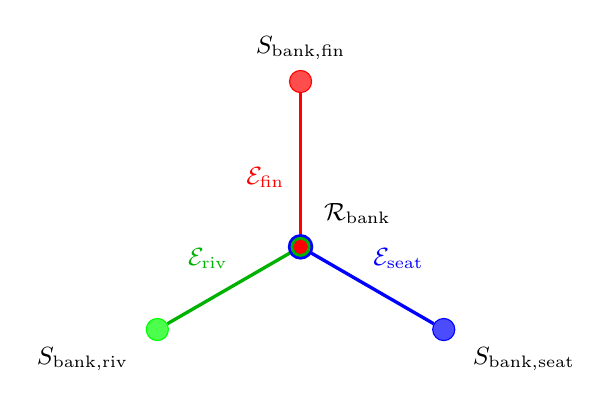
\begin{tikzpicture}[scale=0.5,
    outer/.style={circle, draw, minimum size=8pt,
                  inner sep=0pt, font=\footnotesize},
    lab/.style={font=\small}]
% central shared reference-subspace vertex
\coordinate (c) at (0,0);

\node[lab, above right=7pt] at (c)
{$\mathcal R_{\rm bank}$};

% outer sense-subspace vertices
\node[outer, red, fill=red!70,
      label={[lab]above:
      $S_{{\rm bank},{\rm fin}}$}]
      (fin) at (90:4.2cm) {};

\node[outer, green, fill=green!70,
      label={[lab, xshift=-4pt]below left:
      $S_{{\rm bank},{\rm riv}}$}]
      (riv) at (210:4.2cm) {};

\node[outer, blue, fill=blue!70,
      label={[lab, xshift=4pt]below right:
      $S_{{\rm bank},{\rm seat}}$}]
      (seat) at (330:4.2cm) {};

% hyperedges labelled by context
\draw[very thick, red] (c) --
      node[lab, left=2pt, pos=0.45]
      {$\mathcal E_{\rm fin}$} (fin);

\draw[very thick, green!70!black] (c) --
      node[lab, above left=1pt, pos=0.45]
      {$\mathcal E_{\rm riv}$} (riv);

\draw[very thick, blue] (c) --
      node[lab, above right=1pt, pos=0.45]
      {$\mathcal E_{\rm seat}$} (seat);

% central concentric disks
\filldraw[blue, very thick] (c) circle (8pt);
\filldraw[green!70!black, very thick] (c) circle (6pt);
\filldraw[red, very thick] (c) circle (4pt);
\end{tikzpicture}
\caption{%
Incidence schematic for the lexically ambiguous token ``bank.''  The center is
the single shared reference-subspace vertex
$\mathcal R_{\rm bank}$ and the outer nodes are the financial, river-edge,
and seat/bench sense subspaces in $\mathcal R_{\rm bank}^{\perp}$.  Each
colored arm denotes the displayed two-vertex fragment
$\mathcal E_s=\{\mathcal R_{\rm bank},S_{{\rm bank},s}\}$ associated with
$\Pi_{{\rm bank},s}$; it is not a vector, map, or causal arrow.  The concentric
colors at the center mark membership of the same shared vertex in all three
displayed context-hyperedge fragments.  Additional outcome sectors would
complete each measurement context in a full contextuality hypergraph.
}
\label{fig:reference-subspace}
\end{figure}

\subsection{Relation to dynamic contextual embeddings}
\label{sec:dynamic}

Transformers already handle lexical ambiguity dynamically. The hidden state
$h_\ell(t\mid x)$ of token $t$ at layer $\ell$ depends on context $x$.
The reference-subspace and shared-sector operator hypotheses are not
alternative hardware architectures; they are proposed organizations and
readouts of these observed trajectories.

Given a candidate reference subspace $\mathcal R_t$ and its projector $P_t$,
write
%
\begin{align}
\label{eq:layer-decomp}
h_\ell(t\mid x)
&=P_t h_\ell(t\mid x)+z_\ell(t,x),\\
z_\ell(t,x)&=(I-P_t)h_\ell(t\mid x)
\in\mathcal R_t^\perp.\nonumber
\end{align}
%
The decomposition is automatic; the hypothesis is not. It predicts that
$P_t h_\ell(t\mid x)$ tracks token identity or engagement, while
$z_\ell(t,x)$ carries most sense-disambiguating information. Sense labels
should be more separable in $\mathcal R_t^\perp$ than in the orthogonal
complements of matched control subspaces. For each sense $s$, the projected
states $z_\ell(t,x)$ should also concentrate near the low-dimensional
subspace $S_{t,s}\subset\mathcal R_t^\perp$.

Thus the critical question is not whether contextual embeddings move; they
do. It is whether their sense-relevant movement has a privileged organization
relative to a token-associated reference subspace, and whether conditional
application of $\Pi_{t,s}$ explains that movement better than matched
unstructured projectors.

% ======================================================================
\section{Attention and latent context selection}
\label{sec:attention}
% ======================================================================

A standard attention head computes
%
\begin{equation}
\label{eq:attention}
h'=\sum_j\alpha_j\nu_j,
\qquad
\alpha_j=
\frac{\exp(q_{\rm att}\T k_{{\rm att},j}/\sqrt{d_{\rm head}})}
{\sum_{j'}\exp(q_{\rm att}\T k_{{\rm att},j'}/\sqrt{d_{\rm head}})} .
\end{equation}
%
$q_{\rm att},k_{{\rm att},j}\in\R^{d_{\rm head}}$ are the query and key
vectors of that head, and $\nu_j$ is its value vector.  The local head width
$d_{\rm head}$ is an architectural
quantity, not necessarily the selected carrier dimension $d$ used in the
geometric null model.
Keys and values are produced by different learned maps, so value vectors
are not generally coefficients of a dual basis for the key vectors.
Attention is therefore not literal basis reconstruction.

The useful analogy is softer. Attention routes information: it amplifies
some contextual directions and suppresses others. In the terminology of
Sec.~\ref{sec:reference}, this resembles context-dependent subspace
selection. A literal basis-reconstruction interpretation would require
additional constraints, such as approximately Parseval keys and values
implementing the corresponding dual reconstruction. We do not assume this.

A usable context selector cannot receive the true sense label at inference.
Let learned router logits $\ell_{\theta,s}(x,t)$ depend only on the available
sequence and token state, and define
%
\begin{equation}
\label{eq:context-temp}
p_\theta(s\mid x,t)=
\frac{\exp(\ell_{\theta,s}(x,t)/\tau_{\rm r})}
{\sum_{s'}\exp(\ell_{\theta,s'}(x,t)/\tau_{\rm r})},
\qquad \tau_{\rm r}>0 .
\end{equation}
%
The router may use the illustrative score in Eq.~\eqref{eq:sense-score}, but
need not do so.  Its weights define two possible shared-sector filters:
%
\begin{equation}
\label{eq:soft-observable-embedding}
\begin{aligned}
\bar h_t^{(\Pi)}(x)
&=\sum_s p_\theta(s\mid x,t)\,\Pi_{t,s}h(x),\\
\bar h_t^{(A)}(x)
&=\sum_s p_\theta(s\mid x,t)\,A_{t,s}h(x).
\end{aligned}
\end{equation}
%
Hard selection uses the largest router probability; soft selection uses
Eq.~\eqref{eq:soft-observable-embedding}.  The effective operator
$\sum_s p_\theta(s\mid x,t)\Pi_{t,s}$ is generally not idempotent and hence is
not itself an orthogonal projector.  Attention may supply its routing signal,
but neither the shared sector nor the operator structure follows from standard
attention.  The constrained model must therefore be compared with
parameter-matched mixture-of-experts and unstructured low-rank alternatives.

For an implementable adapter at a chosen layer, let
$Z_{t,s}\in\R^{d\times m_s}$ be a trainable seed matrix such that
$(I-P_t)Z_{t,s}$ has full column rank, and set
$B_{t,s}=\operatorname{orth}((I-P_t)Z_{t,s})$.  Tie the same $Q_t$ across all
$s$, compute the router, and choose
$\bar h_t\in\{\bar h_t^{(\Pi)},\bar h_t^{(A)}\}$ from
Eq.~\eqref{eq:soft-observable-embedding}.  The filtered state may be used as a
diagnostic probe or inserted through the residual update
$h^+=h+\eta U\bar h_t$, where $U\in\R^{d\times d}$ is a learned output map and
$\eta$ is a scalar gate.  The router, bases, spectra, and adapter are then trained on a
language-model or task loss; parameter tying enforces the shared sector and
the factor $(I-P_t)$ enforces transversality.  Held-out evaluation must compare
against adapters with the same ranks and parameter count but no shared-sector
constraint.

% ======================================================================
\section{Discussion}
\label{sec:discussion}
% ======================================================================

The geometric argument now has four deliberately separated layers.  L\'evy's
lemma explains typical near-orthogonality on the sphere; JL explains why a
finite configuration of exponentially many directions can retain its metric
relations in logarithmic dimension; random spherical coding calibrates the
largest overlap; and active-set analysis asks what a decoder can recover.
Each ingredient is standard, but their conjunction exposes the central
tension: quasi-orthogonal code cardinality can grow exponentially while angular
resolution and simultaneous accessibility remain finite.  The discriminating
LLM question is whether training redistributes the unavoidable overlap so that
frequently coactive features incur less held-out interference than isotropic
and activity-matched controls.

The shared-sector operator proposal is logically independent of that null
model.  It asserts that trajectories of some lexically ambiguous tokens admit a
specific constrained organization.  Neither a fitted common subspace nor a
nonzero commutator is sufficient evidence.  Evidence requires generalization
to held-out contexts and an advantage over equally expressive unstructured
projectors or mixture models.

\subsection{Relation to superposition and sparse autoencoders}
\label{sec:superposition}

The superposition hypothesis holds that neural networks may represent more
features than they have neurons by using nonorthogonal directions with sparse
activity~\cite{elhage2022superposition,bricken2023monosemanticity}.  The null
model separates dictionary coexistence from simultaneous linear readout.  In
the isotropic, weak-dependence model, many directions can coexist while a
fixed-target correlation decoder accumulates interference of scale
$\sqrt{k/d}$.  Sparse activity controls that interference for this decoder;
it is not asserted to be universally necessary for structured dictionaries or
nonlinear recovery.

Sparse autoencoders (SAEs) give a concrete empirical interface. They
approximate layer activations as sparse expansions over learned decoder
directions, making the $w_i$ of Eq.~\eqref{eq:hidden} measurable
objects rather than hypothetical features. Recent work has scaled SAEs,
studied SAE feature geometry, and automated interpretation of large
numbers of latents~\cite{gao2025scaling,li2025geometry,paulo2025automatically,shu2025survey}. In the
present framework, SAE decoder directions make the L\'evy/JL calibration and
coactivation-weighted diagnostic measurable, while sense-conditioned SAE
activation clusters can test the stronger reference-subspace hypothesis.

\subsection{Limitations}
\label{sec:limitations}

The framework can fail in several ways.

First, L\'evy's lemma controls a regular probe or a fixed overlap; mutual
quasi-orthogonality of a finite family additionally requires a union bound or
code construction.  JL supplies a constructive exponential scale, not a hard
upper bound on spherical codes.  The deterministic Welch bound constrains a
specified $\Msem$-vector dictionary, while Eq.~\eqref{eq:max-overlap} describes
an independent isotropic ensemble.  None is a semantic impossibility theorem.

Second, the double exponential is conditional on fixed $q>1$, fixed
$0<\varepsilon<1$, and access to a full carrier with tensor dimension
$d=q^n$.  Sequence length, compositional language, or the existence of many
possible contexts does not by itself give a Transformer residual-stream tensor
product.  Restriction to product vectors or another low-complexity family may
remove the second amplification.  Without the full-carrier premise, the
ambient code has an existence lower bound exponential, not doubly
exponential, in measured $d$.

Third, the nominal layer width need not equal the selected carrier rank $d$.
Contextual embeddings can be anisotropic, and the occupied carrier can vary
strongly by layer and training regime
\cite{ethayarajh2019,gao2019representation,mu2018allbutthetop,razzhigaev2024shape}. Whitening and
related postprocessing can partially restore isotropic geometry
\cite{gao2019representation,mu2018allbutthetop,su2021whitening}. At the same time, anisotropy should not
be treated as an automatic or universal property of all Transformer
representations~\cite{machina2024anisotropy}. The rule used to select or
whiten a $d$-dimensional carrier must therefore be reported. Whitening also
changes the metric in which overlaps are measured, and the covariance spectrum
may contain information not summarized by one rank. We do not introduce a
second dimension symbol, but $d$ is protocol-dependent rather than an
intrinsic semantic constant.

Fourth, $\Msem$ depends on the feature-extraction, normalization, and
duplicate-removal rules.  A claimed departure from the null may instead expose
a poor dictionary, dependence among samples, finite-size effects, or a changed
metric.  These alternatives must be checked before attributing the departure
to learned semantic organization.

Fifth, the reference-subspace pattern may simply be descriptively wrong.
Trained models may represent lexical ambiguity without a preferred token-associated
direction or subspace.  A low-rank fit found after inspecting test labels is
not evidence; ranks, candidate references, and routers must be selected on
training data and evaluated out of sample.

Sixth, the law $\sint\sim\sqrt{k/d}$ concerns a fixed-target correlation
readout with random-like directions and weakly correlated signs or amplitudes.
It is neither a joint sparse-recovery theorem nor a universal equality.
Structured dictionaries, nonlinear decoders, multiple comparisons over
inactive features, and correlated errors can change the scaling.

The coactivation energy in Eq.~\eqref{eq:int-energy} is likewise a diagonal
proxy.  If interference contributions from distinct features are correlated,
the full importance-weighted squared error contains additional covariance
terms and must be estimated directly.

Finally, the operator model has choices: the candidate reference subspace
$\mathcal R_t$, the router, the local ranks, and any spectra in
Eq.~\eqref{eq:context-observable}.  The true sense label cannot be supplied to
the router at test time.  Eigenvalues are not identified by subspaces alone,
and a fitted nonzero commutator is generic.  These choices add evidence only
through held-out prediction, compression, or prespecified order effects.

\subsection{Empirical predictions}
\label{sec:predictions}

The key empirical task is to distinguish the applicability of the
L\'evy/JL geometry from three stronger semantic hypotheses.

\emph{Geometric calibration (not a semantic claim).}
For a dictionary independently established to be overcomplete, compare its
coherence, overlap distribution, and fixed-target readout error with isotropic
and activity-matched controls.  Agreement with Eq.~\eqref{eq:max-overlap} is a
baseline result, not evidence that overcompleteness is useful; departure from
it must be diagnosed before being called learned structure.  JL itself is a
theorem; the empirical question is whether task-relevant geometry and readout
survive projection near its logarithmic dimension scale.

\emph{Claim A: privileged token reference subspace.}
For a lexically ambiguous token $t$, there exists a privileged token-associated
subspace $\mathcal R_t$ such that sense-relevant variation is better
exposed in $\mathcal R_t^\perp$ than in the orthogonal complements of
matched control subspaces of the same dimension.

\emph{Claim B: low-dimensional sense subspaces.}
Within $\mathcal R_t^\perp$, sense-conditioned states admit a cross-validated
low-rank description that predicts or compresses held-out states better than
shuffled-label, ordinary clustering, and matched-subspace controls.  Related
polysemous senses need not have minimal cross-sense coherence.

\emph{Claim C: shared-sector class operators.}
A non-oracular router and class-conditioned projectors $\Pi_{t,s}$ sharing $P_t$ improve
held-out contextual prediction or compression relative to parameter-matched
unstructured projectors and mixture-of-experts models.  A commutator matters
only if it predicts order effects defined independently of the fitted
operators.

These claims can fail independently.  The geometric calibration can hold while all
three structural claims fail.  Claim A can hold while sense information
remains high-dimensional.  Claim B can hold relative to a non-token-associated
subspace, in which case Claim A fails.  Claims A and B can hold even if the
operator constraint in Claim C adds no predictive value.

The following tests separate the possibilities.

\begin{enumerate}
\item \emph{L\'evy/random-code calibration.}
Fix the carrier metric, spectral threshold or whitening rule, feature extractor,
and duplicate criterion before evaluation.  Report the selected rank $d$,
dictionary size $\Msem$, maximum coherence, the full overlap distribution, and
active-set statistics.  Compare with the Welch floor, isotropic dictionaries,
and controls matched for marginal activity and coactivation.  Treat
Eq.~\eqref{eq:max-overlap} as a finite-sample null prediction, not a pass/fail
capacity test.  Also compare the signed pairwise distribution with the
independently isotropic variance $1/d$; deviations may reflect dependence,
anisotropy, extraction choices, or learned alignment.

\item \emph{JL projection-stability test.}
Fix a finite evaluation set of $\Msem$ normalized directions or contextual
states, include the origin, and prespecify a relative squared-distance
distortion $\delta_{\rm JL}$.  Project to $d_{\rm proj}$ dimensions using
frozen random maps and measure pairwise distortion and held-out task
performance as $d_{\rm proj}$ varies.  JL predicts metric preservation on the
scale $d_{\rm proj}=O(\!\delta_{\rm JL}^{-2}\log(\Msem+1))$; preservation of
semantic performance is the additional empirical question.  Compare random
Gaussian or orthogonal maps with learned low-rank maps at the same
$d_{\rm proj}$.

\item \emph{Reference-subspace test.}
For a lexically ambiguous token, choose candidate reference subspaces generated
by the mean contextual embedding, a static input embedding explicitly mapped
into the same layer carrier,
learned token-specific directions, or a low-dimensional combination of
these. Project layer states as in Eq.~\eqref{eq:layer-decomp}. Sense labels
should be better separated in $\mathcal R_t^\perp$ than in orthogonal
complements obtained after ordinary centering, token-mean subtraction,
top-principal-component removal, and random, frequency-matched, or
layer-matched control subspaces of the same rank.  Compare held-out
classification, compression, or incremental mutual information, with
permutation over sense labels and bootstrap over token instances.

\item \emph{Operational subspace test.}
For each sense $s$, collect projected states
$z_\ell(t,x)\in\mathcal R_t^\perp$ and estimate a low-rank subspace by PCA or
probabilistic factor analysis. Select $m_s$ without test-label leakage and use
an orthonormal basis $B_{t,s}$.  Evaluate held-out reconstruction and sense
prediction against shuffled labels, ordinary supervised subspaces, and
unsupervised clustering of equal rank.  Report
$\opnorm{B_{t,s}\T B_{t,s'}}$ descriptively, without assuming related senses
must be nearly orthogonal.

\item \emph{Reference-versus-sense readout test.}
Linear probes trained on $z_\ell(t,x)$ should perform comparably to
probes trained on the full state $h_\ell(t\mid x)$, while probes
restricted to the reference component $P_t h_\ell(t\mid x)$ should provide
less incremental sense information after frequency, syntax, and sense-prior
controls.  Near-chance performance is not required because the reference
component may legitimately retain correlated information.

\item \emph{Shared-sector operator test.}
Fit $P_t$, $B_{t,s}$, $A_{t,s}$, and the router on training sequences, then evaluate
Eq.~\eqref{eq:soft-observable-embedding} without true sense labels on held-out
instances. Compare with unconstrained low-rank projectors, ordinary contextual
probes, parameter-matched mixture-of-experts models, and shuffled class or
sense labels.  If an order claim is made, define the sequential linguistic or model
intervention independently; then ask whether
$\opnorm{[\Pi_{t,s},\Pi_{t,s'}]}$ predicts the measured asymmetry.  Merely
obtaining a nonzero commutator does not pass the test.

\item \emph{Synthetic concurrency degradation.}
At a fixed layer, inject controlled superpositions
%
\begin{equation}
h_k=h_0+\lambda\sum_{j=1}^k x_j w_j,
\end{equation}
%
where $h_0$ is a held-out baseline activation, the $w_j$ are independently
chosen unit injection directions, the coefficients $x_j$ are independent,
centered, and unit-variance, and $\lambda$ controls injection amplitude.  The
directions may come, for example, from SAE decoder directions or frozen linear
probes. As $k$ increases, readout
should degrade smoothly on the scale $\sqrt{k/d}$ for random-like
directions under the specified correlation decoder.  Include norm-preserving,
random-direction, activation-frequency, and out-of-distribution controls;
degradation by itself does not validate semantic superposition.

\item \emph{Coactivation-dependent geometry.}
At matched marginal activation frequency, feature similarity, SAE
reconstruction error, amplitude, and task relevance, important frequently
coactive features should contribute less to Eq.~\eqref{eq:int-energy} than
activity-matched controls.  This tests learned redistribution of interference,
independently of the reference-subspace hypothesis.
\end{enumerate}

\subsection{Scope of the quantum analogy}
\label{sec:quantum}

The analogy to quantum contextuality is structural and limited.  In the
proposed construction, every $\Pi_{t,s}$ acts identically on the invariant
subspace $\mathcal R_t$.  Under the spectral-separation condition stated after
Eq.~\eqref{eq:context-observable}, the observables $A_{t,s}$ additionally share
$P_t$ as the spectral projector of $\lambda_t$.  The shared term cancels from
the commutator, so it is the relative geometry of the sense sectors that may
produce order dependence.  Figure~\ref{fig:reference-subspace}
records the displayed incidence pattern; omitted complementary outcome sectors
would be required to complete each measurement context in a full contextuality
hypergraph.  Equations~\eqref{eq:context-projector}--
\eqref{eq:context-observable} provide the corresponding operator
parameterization.  Vectors, subspaces, projectors, and observables are distinct
mathematical types.

Quantum contextuality has the force of no-go theorems such as
Kochen--Specker~\cite{specker-60,kochen1}; no analogous theorem is claimed
here for semantic embeddings.  Real symmetric matrices can be noncommuting
while still being stored and evaluated on an ordinary classical computer, and
generic fitted projectors are commonly noncommuting.  Thus noncommutativity by
itself supplies neither a semantic result, Born probabilities, nor physical
quantumness.

Three levels of analysis should not be conflated.
%
\begin{enumerate}
\item \emph{Classical high-dimensional representation.}
A present-day Transformer carries real-valued hidden states through
attention, nonlinear feed-forward maps, residual connections, and
normalization.  Concentration, quasi-orthogonality, feature superposition,
dynamic embeddings, and finite readout are all available at this level.
None requires quantum probability or quantum hardware.

\item \emph{Quantum-like semantic or contextual formalism.}
States, contexts, bases, interference terms, noncommuting questions, or
measurement-like updates may be used as an abstract model of meaning even
when the implementation remains classical.  The relevant issue is not the
vocabulary but whether this extra structure improves compression,
explanation, or prediction relative to an ordinary contextual embedding
model.

\item \emph{Genuine quantum machine learning or quantum attention.}
Here semantic states would be encoded in qubits or other physical quantum
degrees of freedom, intermediate evolution would be unitary, phase would
affect interference, and measurement would follow quantum probability.  A
standard Transformer does none of these things.
\end{enumerate}
%

The random-dictionary and linear-readout baselines belong entirely to the first
level.  Shared-sector projection is also an ordinary classical computation.
The proposal earns the stronger quantum-like interpretation only if its
operator constraints or prespecified order effects improve prediction,
compression, or explanation relative to equally expressive classical
baselines.  Even a positive result would support a useful formalism, not
physical quantum computation; phase-sensitive dynamics and Born-rule
measurement remain absent.

The conditional double exponential has its most direct realization in a
full tensor-product Hilbert space, where $n$ local $q$-level factors give
$d=q^n$ before quasi-orthogonal packing is considered.  This is a statement
about composition and finite angular resolution, not a signature of physical
quantumness; classical tensor-product feature spaces can exhibit the same
counting.  Conversely, importing $d=q^n$ into an ordinary LLM merely because
language is compositional would be unwarranted.  The carrier factorization and
access to the full carrier, rather than only product states or another
low-complexity manifold, must be demonstrated.

The dimension of $\mathcal R_t$ is also explicit. In Hilbert-space quantum
logic, two or more contexts may share one spectral sector, or several; a
four-dimensional example has two contexts with two common observables
~\cite{svozil:040102}. The semantic
analogue is $\dim(\mathcal R_t)=p$: $p=1$ is the simplest case, while
$p>1$ permits several token-associated reference directions. In every case,
sense-specific information is hypothesized to occupy subspaces of
$\mathcal R_t^\perp$.

% ======================================================================
\section{Conclusion}
\label{sec:conclusion}
% ======================================================================

The central geometric conclusion is an abundance--resolution tradeoff.
L\'evy's lemma says that regular probes concentrate on a high-dimensional
sphere and, in particular, that almost every direction has small overlap with
any fixed direction.  Johnson--Lindenstrauss supplies the complementary
finite-set statement: logarithmic exact dimension suffices to retain the
pairwise geometry of many points.  Applied constructively to an orthogonal
family, it yields quasi-orthogonal codes of size
$M_\varepsilon(d)\geq\exp(c\varepsilon^2d)$ for fixed tolerance and
sufficiently large $d$.  Direct random spherical coding recovers the same
exponential scale, and the exact complex-Haar law gives
Eq.~\eqref{eq:complex-code}, whereas the Welch bound gives the hard
coherence floor for any specified overcomplete family.  These are distinct
views---typicality, finite-set embedding, random construction, and
deterministic obstruction---of the same quasi-dimensional geometry.

A genuine double exponential requires two amplifications.  If an independently
justified, fully accessible tensor-product carrier gives $d=q^n$, then for
fixed $q>1$ and fixed $0<\varepsilon<1$ the quasi-orthogonal code cardinality
has an existence lower bound of the form
$\exp(c\varepsilon^2q^n)$, doubly exponential in the factor count $n$.  The
claim need not survive restriction to product vectors or another
low-complexity state family.  Nothing in L\'evy's or the JL lemma alone makes
the number of semantic directions doubly exponential in an ordinary LLM
width.  For a Transformer
residual stream treated simply as $\R^d$, the supported conclusion is
an ambient-code existence lower bound exponential in measured $d$;
tensor-product growth must be established separately.

The same high-dimensional geometry that permits large codes also concentrates
typical angles and limits access.  In the small-overlap regime
$\log\Msem\ll d$, an independently sampled isotropic dictionary has a
largest-overlap scale of order $2\sqrt{\log\Msem/d}$, and a random-like active set produces fixed-target
correlation-readout interference of order $\sqrt{k/d}$.  The substantive
semantic hypothesis concerns where the remaining overlap is placed: important
features that frequently coactivate should contribute less
coactivation-weighted interference than activity-, amplitude-, and
importance-matched controls.  This connects the L\'evy/JL code-cardinality
picture to
observable readout rather than equating code cardinality with usable meaning.

The second proposal is a constrained operator model of lexical ambiguity.
Class-conditioned projectors share a token-associated invariant sector and differ on
low-dimensional sense subspaces in its orthogonal complement.  Conditional
projection or observable filtering yields a class-conditioned embedding, and a
learned non-oracular router selects or mixes classes from the observed context.
The common projector does not
cause noncommutativity, and a nonzero fitted commutator has no evidential force
by itself.  The model succeeds only if the shared-sector constraint improves
held-out prediction or compression over parameter-matched unstructured models,
or if its commutators predict independently specified order effects.

The geometric calibration, coactivation hypothesis, and shared-sector model
can fail independently.  The construction is quantum-inspired, not a claim
that a Transformer is a quantum device: it uses real matrices on classical
hardware and introduces no Born rule, unitary dynamics, or physical
measurement.  Quantum terminology is earned only if the constrained operator
structure provides additional held-out explanatory or predictive value.

\appendix

% ======================================================================
\section{Minimal formalization of the three computational loops}
\label{app:llm-loops}
% ======================================================================

The following subsections correspond one-to-one to
Secs.~\ref{sec:prose-training}--\ref{sec:prose-online}.  Let $\Theta$ collect
all persistent real-valued model parameters, let $\mathcal V$ be the token
vocabulary, and let $\mathsf{Tok}$ and $\mathsf{Detok}$ denote tokenization and
detokenization.  Hidden states lie in the finite real inner-product space
$\R^d$.

\subsection{Creating the weights}
\label{app:training}

For a training string $\sigma$, write
%
\begin{align}
x_{1:T_\sigma}^{(\sigma)}
&=\mathsf{Tok}(\sigma),
&e_i^{(\sigma)}
&=E_{\rm tok}[x_i^{(\sigma)}]\in\R^d,
\nonumber\\
h_{1:T_\sigma}^{(L,\sigma)}
&=F_\Theta\!\left(e_{1:T_\sigma}^{(\sigma)};1{:}T_\sigma\right).
\label{eq:app-forward-map}
\end{align}
%
Here $E_{\rm tok}$ is the learned embedding table, and $1{:}T_\sigma$ records
that the forward map receives positional information.  The latter may be
additive, rotary, or relative.  The map $F_\Theta$ contains causal
self-attention of the form already displayed in Eq.~\eqref{eq:attention}, as
well as residual, normalization, multi-head, and feed-forward operations.
During this forward pass $\Theta$ is fixed.  The attention coefficients and
hidden states computed by $F_\Theta$ are transient.

With vocabulary logits
$g_{\sigma,i}=W_{\rm out}h_i^{(L,\sigma)}+b$, next-token training may be
written schematically as
%
\begin{align}
\widehat{\mathcal L}_{\mathcal B_r}(\Theta)
&=-\sum_{\sigma\in\mathcal B_r}
\sum_{i=1}^{T_\sigma-1}
\log\!\left[
\operatorname{softmax}(g_{\sigma,i})_{x_{i+1}^{(\sigma)}}
\right],\nonumber\\
\Theta^{(r+1)}
&=\operatorname{Opt}\!\left(
\Theta^{(r)},
\nabla_\Theta\widehat{\mathcal L}_{\mathcal B_r}
(\Theta^{(r)})
\right).
\label{eq:app-training-update}
\end{align}
%
Here $\mathcal B_r$ is the minibatch at optimization step $r$.  Equation
\eqref{eq:app-forward-map} changes activations during a forward pass;
Eq.~\eqref{eq:app-training-update} changes persistent weights between passes.

\subsection{Generating the output}
\label{app:generation}

Let $u_{1:m}=\mathsf{Tok}(\sigma_{\rm prompt})$ and let $\Theta^\star$ denote the
fixed deployed parameters.  At generation step $j\geq m$, the forward map
returns logits $g_j(\Theta^\star;u_{1:j})$, and for
$\tau_{\rm dec}>0$ a temperature-scaled sampling distribution is
%
\begin{align}
\pi_j(a)
&=
\frac{\exp\!\left[g_{j,a}(\Theta^\star;u_{1:j})/\tau_{\rm dec}\right]}
{\sum_{b\in\mathcal V}
\exp\!\left[g_{j,b}(\Theta^\star;u_{1:j})/\tau_{\rm dec}\right]},
\qquad a\in\mathcal V,
\nonumber\\
u_{j+1}&\sim\pi_j,
\nonumber\\
u_{1:j+1}&=(u_{1:j},u_{j+1}).
\label{eq:app-generation}
\end{align}
%
A greedy or truncated decoding rule may replace direct sampling.  If
generation stops at $J$, the returned string is
$\widehat s=\mathsf{Detok}(u_{m+1:J})$.  The prefix and all context-dependent
states change with $j$, but $\Theta^\star$ does not.  A key--value cache stores
previously computed activations and likewise leaves $\Theta^\star$ unchanged.

\subsection{Recursive adaptation, alignment, and hallucination}
\label{app:online}

Post-training alignment first produces a deployed starting point
$\Theta_{\rm align}:=\Theta^{(0)}=
\operatorname{Align}(\Theta_{\rm base};\mathcal D_{\rm inst},
\mathcal D_{\rm pref})$ from instruction and preference data.  Genuine online
adaptation adds a parameter update after interaction round $r$:
%
\begin{equation}
\label{eq:app-online-update}
\Theta^{(r+1)}
=\Theta^{(r)}-\eta_r\mathcal P_r^{(\Theta)}
\nabla_\Theta\mathcal J_r
(\Theta^{(r)};\mathcal B_r),
\qquad \eta_r>0.
\end{equation}
%
Here $\mathcal B_r$ is verified adaptation data, $\mathcal J_r$ is its declared
adaptation objective, and $\mathcal P_r^{(\Theta)}$ is a mask or projection in
parameter space.  Setting $\mathcal P_r^{(\Theta)}=0$ recovers ordinary
frozen-weight inference; restricting it to adapter coordinates confines the
update to those parameters; the identity permits a full update.  Boundedness
additionally requires clipping, a trust region, or an explicit norm bound.  An
external-memory update instead has
$m_{r+1}=U_{\rm mem}(m_r,\iota_r)$, where the interaction record $\iota_r$ may
contain the round-$r$ input, response, tool results, and verified feedback.
It leaves $\Theta$ fixed and is therefore not
Eq.~\eqref{eq:app-online-update}.

Finally, let $H(\Theta;\mathcal Q,\mathcal G,\mathcal D)$ be a prespecified
held-out rate of unsupported claims for prompt distribution $\mathcal Q$,
grounding condition $\mathcal G$, and decoding rule $\mathcal D$.  The causal
contrast requested in Sec.~\ref{sec:prose-online} is
%
\begin{equation}
\label{eq:app-hallucination-test}
\Delta_{\rm hall}^{\rm align}
=H(\Theta_{\rm align};\mathcal Q,\mathcal G,\mathcal D)
-H(\Theta_{\rm ctrl};\mathcal Q,\mathcal G,\mathcal D).
\end{equation}
%
The control $\Theta_{\rm ctrl}$ starts from the same base and is matched in
data exposure, optimization and compute budget, and random seeds, except for
the declared alignment intervention.  One may set
$\Theta_{\rm ctrl}=\Theta_{\rm base}$ only when ``no post-training'' is the
explicit control condition.  Coverage and abstention must be reported beside
$H$, since universal refusal could otherwise lower the unsupported-claim rate
without adding knowledge.

The hypothesis that alignment increases hallucination in the declared regime
is $\Delta_{\rm hall}^{\rm align}>0$; reduction corresponds to a negative
value.  Nothing in the formalism fixes the sign.  A cumulative online update
is tested against a frozen control exposed to the same interaction stream,
not merely against its own earlier parameter snapshot.

\begin{acknowledgments}
OpenAI Codex (GPT-5) was used to assist with literature organization, \LaTeX{}
editing, and checks of derivations.  The author specified the scientific
direction and prompts; model output retained in the manuscript was checked
against the cited sources and explicit calculations.  The author accepts full
responsibility for the final text.

This research was funded in part by the Austrian Science Fund (FWF), grant DOI
\href{https://doi.org/10.55776/PIN5424624}{10.55776/PIN5424624}.
The author also acknowledges support from the TU Wien Bibliothek Open Access
Funding Programme.

The author declares no conflict of interest.
\end{acknowledgments}

\clearpage

\bibliography{svozil}

\end{document}
